\documentclass{report}
\usepackage[italian]{babel}
\usepackage[utf8]{inputenc}
\usepackage{natbib}
\usepackage{graphicx}
\usepackage{cleveref}
\usepackage{dirtree}
\usepackage{xcolor}

\definecolor{codegray}{gray}{0.925}
\newcommand{\code}[1]{\colorbox{codegray}{\texttt{\detokenize{#1}}}}
\newenvironment{codeblock}[1]{\colorbox{codegray}{\texttt{\detokenize{#1}}}}

\title{
    MyWaste \\
    \large Applicazioni e Servizi Web
}

\author{Federico Pettinari - 988120 \{federico.pettinari2@studio.unibo.it\}\\
Hamado Dene - 973128 \{hamado.dene@studio.unibo.it\}}
\date{\today}

\begin{document}

\maketitle
\section{Introduzione}
%Introduzione \citep{adams1995hitchhiker}
Lo scopo del progetto è la realizzazione di un'applicazione web per la gestione dei dati dei rifiuti cittadini ed i relativi conferimenti,
in modo che ogni cittadino possa sapere (anche in tempo reale) la quantità ed il costo dei rifiuti prodotti.
A questo scopo si presume che ogni cassonetto per la raccolta differenziata sia dotato di lettore RFID per poterne identificare
il padrone in modo automatico.

\section{Requisiti}
\begin{itemize}
    \item Progettare e sviluppare una web app per la visualizzazione e gestione dei dati sui rifiuti cittadini
    \item I cassonetti sono dotati di sensore di peso e lettore rfid per identificare l’utente che sta conferendo i rifiuti
    \item La piattaforma deve calcolare il costo mensile in funzione del tipo di rifiuto e peso.
    \item Deve mostrare la notifica del conferimento all’utente
    \item Deve mostrare grafici statistici sul conferimento
\end{itemize}

\section{Design}
\subsection{Architettura}
L'architettura è raffigurata in \Cref{fig:arch}.
Ogni richiesta HTTP viene ricevuta e smistata dal reverse proxy.
Le chiamate che iniziano con /api vengono passate al backend, mentre le altre al frontend.
Questo aiuta a separare frontend e backend in modo trasparente e senza bisogno di utilizzare Cross-Origin Resource Sharing (CORS).

\begin{figure}[h!]
\centering
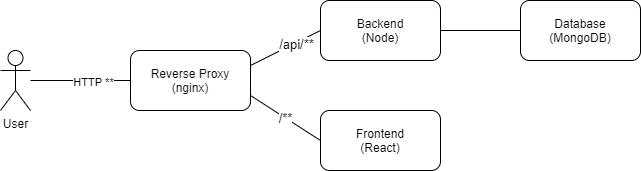
\includegraphics[width=\textwidth]{arch}
\caption{Architettura}
\label{fig:arch}
\end{figure}

\subsection{Database}
Il modello del database è semplice e raffigurato in \Cref{fig:db}. L'applicazione può avere un numero variabile di account.
Ad ogni account sono associate le proprie notifiche e conferimenti (Waste). Un account oltre ai dati di identificazione
(email e password), ha un ruolo (role) per distinguere amministratori da utenti. Per ogni conferimento vengono memorizzati
la data, il tipo di spazzatura (es. plastica o carta) e la quantità. Per ogni notifica vengono memorizzati la data di creazione,
una flag per sapere se è stata letta, ed il tipo e quantità per i conferimenti.
\begin{figure}[h!]
    \centering
    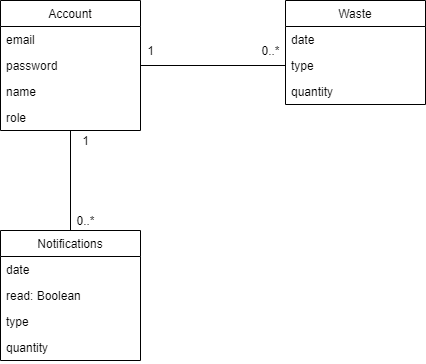
\includegraphics[width=\textwidth]{db}
    \caption{Modello del database}
    \label{fig:db}
\end{figure}

\subsection{Interfaccia utente}
TODO. Mockup....

\section{Tecnologie}
Il progetto utilizza le seguenti tecnologie:
\begin{itemize}
    \item Github Actions - per continous integration
    \item Docker - per disaccoppiare il software dal sistema operativo e facilitarne il porting ed installazione.
    \item nginx - utilizzato come reverse proxy
    \item MongoDB - database non relazionale di documenti
    \item Node - come server web sia per frontend e backend
    \item Express - libreria per gestire chiamate e route HTTP
    \item Mongoose - come libreria di object modeling per mongodb
    \item Mocha e Supertest - per testing automatizzato nel backend
    \item mongodb-memory-server - per utilizzare un database mongodb in memoria, in modo da velocizzare l'esecuzione dei test
    \item bcrypt - per criptare le password degli utenti ai fini di sicurezza
    \item express-jwt - libreria per facilitare l'uso di tokens JWT utilizzati nel sistema di login utente
    \item Nodemon - tool che riavvia le applicazioni Node ad ogni modifica del sorgente
    per velocizzarne lo sviluppo e debugging
    \item React - framework per frontend
    \item SCSS - libreria pre-processore di CSS per facilitarne il riuso
\end{itemize}

\section{Codice}
Solo aspetti rilevanti.

\section{Test}
\subsection{Codice}
A livello di codice sono state adottate tecniche di continous integration con le Github Actions ed il framework e librerie di testing
Mocha e Supertest.
Ad ogni push di codice viene eseguita automaticamente la suite di testing opportunatamente creata.
Questo sistema aiuta a prevenire regressioni e facilita la manutenzione.
\subsection{Interfaccia}
Il progetto è stato testato in modalità Cognitive Walkthrough con i seguenti task:
\dirtree{%
.1 Visualizzazione e comprensione della propria dashboard.
    .2 Login.
    .2 Individuazione dashboard.
    .2 Comprensione.
        .3 Individuazione costo mensile.
        .3 Individuazione quantità di spazzatura conferita in un determinato mese.
        .3 Individuazione numero, data, e dettagli dei conferimenti avvenuti.
    .2 Logout.
.1 Ricevuta notifica a seguito di un conferimento.
.1 Visualizzazione e comprensione dashboard per amministratori.
    .2 Individuazione lista utenti.
    .2 Individuazione quantità e ripartizione dei vari tipi di spazzatura in un determinato mese.
.1 Creazione di un nuovo utente.
    2. Gestione dei casi con input non valido (es{.} in caso di dati duplicati l'utente è in grado di capire cosa fare?).
}
Infine, una volta creato un prototipo funzionante e risolti i primi problemi individuati dal team di sviluppo,
sono stati effettuati Usability Tests con 5 potenziali veri utenti. Ad ognuno di essi è stato chiesto di effettuare i task
sopracitati senza però essere messi al corrente degli step intermedi. In questo modo è stato possibile osservare quanto fosse
intuitiva l'interfaccia ed apportare migliorie.
TODO: descrivere migliorie


\section{Deployment}
%Rilascio, installazione e messa in funzione.
Il progetto può essere scaricato con \code{git clone https://github.com/fedpet/aws-project.git} ed avviato con
\code{docker compose up} nella sua cartella root. A questo punto basterà aprire localhost con un browser web per
vederne l'interfaccia.

TODO: rilascio di immagini docker senza clonare la repo

\section{Conclusioni}
Conclusioni

\bibliographystyle{plain}
\bibliography{references}
\end{document}
